\documentclass[a4paper, 12pt]{book}

\usepackage[T1]{fontenc}
\usepackage[utf8]{inputenc}
\usepackage[italian]{babel}
\usepackage[colorlinks]{hyperref}
\usepackage{listings}
\usepackage{xcolor}
\usepackage{graphicx}
\usepackage{multirow}

\definecolor{codegreen}{rgb}{0,0.6,0}
\definecolor{codegray}{rgb}{0.5,0.5,0.5}
\definecolor{codepurple}{rgb}{0.58,0,0.82}
\definecolor{backcolour}{rgb}{0.95,0.95,0.92}

\lstdefinestyle{mystyle}{
    backgroundcolor=\color{backcolour},   
    commentstyle=\color{codegreen},
    keywordstyle=\color{violet},
    numberstyle=\tiny\color{codegray},
    stringstyle=\color{codepurple},
    basicstyle=\ttfamily\footnotesize,
    breakatwhitespace=false,         
    breaklines=true,                 
    captionpos=b,                    
    keepspaces=true,                 
    numbers=left,                    
    numbersep=5pt,                  
    showspaces=false,                
    showstringspaces=false,
    showtabs=false,                  
    tabsize=2
}

\lstset{style=mystyle}

\title{Laboratorio Sistemi Operativi}
\author{Giovanni Tosini}
\date{}

\begin{document}

    \begin{titlepage}
        \maketitle
    \end{titlepage}

    \frontmatter
    \tableofcontents
    \mainmatter

    \chapter{Processi e programmi}

    Un processo è un'istanza di un programma eseguito.
    Come viene creato, il \textbf{Kernel} gli associa
    una certa struttura di memoria.
    \begin{description}
        \item[Program code:] segmento in sola lettura  contenente istruzioni in linguaggio macchina;
        \item[Initialized data:] segmento contenente variabili globali e statiche;
        \item[Uninitialized data:] segmento contenente variabili globali e statiche \textbf{non} inizializzate;
        \item[Heap:] segmento contenente variabili allocate dinamicamente;
        \item[Stack:] segmento contenente gli argomenti e le variabili interne delle funzioni.    
    \end{description}
    Una delle strutture dati di supporto è il \textbf{file
    descriptor table}, conterrà tutti i file che il 
    processo aprirà. Ogni processo contiene già 3 
    \textbf{file descriptor} associati ad esso:
    \begin{enumerate}
        \item Standard input
        \item Standard output
        \item Standard error
    \end{enumerate}
    Ogni successivo file aperto verrà identificato con 
    il valore minore disponibile. Il file descriptor
    table è visibile \textbf{solo} a runtime.

    \chapter{System call}

    Sono un punto di ingresso verso il Kernel, vengono 
    utilizzate per richiedere dei servizi. Dallo User Level 
    verranno fatte delle chiamate alla System Call 
    Interface che a sua volta comunicherà al Kernel.

    \section{Gestione degli errori delle System Call}

    Nella sezione ERRORS del comando \verb|man| si possono trovare
    tutti i possibili valori di ritorno di errore di una 
    System Call. Tuttavia è possibile usare la variabile 
    \verb|errno| accedibile tramite l'uso della libreria
    \verb|<errno.h>|. Ci permetterà di sapere l'errore 
    effettivo causato in base al valore salvato al suo 
    interno.

    Esempio:
    \begin{lstlisting}[language=C]
        #include <errno.h>
        ...
        //system call to open a file
        fd = open(pathname, flags, mode);
        //Begin code handling errors
        if(fd == -1){
            if(errno == EACCES){
                //Handling not allowed access to the file
            }
            else{
                //Some other error occured
            }
        }
        //End code handling errors
        ...
    \end{lstlisting}
    La maggior parte delle system call ritorna un -1 
    o \verb|NULL| Pointer in caso di errore, alcune però 
    usano il -1 come valore di ritorno anche in caso di 
    \textbf{non} errore. Qui l'uso di \verb|errno| acquista 
    ulteriore valore. Esempio:
    \begin{lstlisting}[language=C]
        #include <sys/resource.h>
        ... 
        //Reset the errno variable to 0
        errno = 0;
        //System call getpriority gets the nice value of a process 
        nice = getpriority(which, who);
        if((nice == -1) && (errno != 0)){
            //Handling getpriority errors
        }
        ...        
    \end{lstlisting}
    
    Esistono altre funzioni che aiutano a gestire gli 
    errori, come la funzione \verb|perror()| che stampa 
    su standard error la stringa che le viene fornita.
    Esempio:
    \begin{lstlisting}[language=C]
        #include <stdio.h>
        ... 
        //System call to open a file
        fd = open(pathname, flags, mode);
        if(fd == -1){
            perror("<Open>");
            //System call to kill the current process
            exit(EXIT_FAILURE);
        }
        ...
    \end{lstlisting}
    L'output sarà:
    \begin{lstlisting}[language=C]
        <Open>: No such file or directory
    \end{lstlisting}
    
    La libreria \verb|string.h| fornisce la funzione 
    \verb|strerror()| che prende in input il valore di 
    \verb|errno| e stampa l'errore effettivo. Esempio:
    \begin{lstlisting}[language=C]
        #include <stdio.h>
        ... 
        //System call to open a file
        fd = open(path, flags, mode);
        if(fd == -1){
            printf("Error opening (%s): \n\t%s\n", path, strerror(errno));
            //System call to kill the current process
            exit(EXIT_FAILURE);
        }
        ...
    \end{lstlisting}
    L'output sarà il seguente:
    \begin{lstlisting}[language=C]
        Error opening (myFile.txt):
            No such file or directory        
    \end{lstlisting}

    \chapter{Kernel data types}

    Sono delle \verb|typedef| di tipi normali C, necessari
    per ovviare problemi di portabilità, per esempio 
    il \verb|pid_t| usato per identificare il process ID
    di un processo non è altro che un tipo definito come 
    \verb|typedef int pid_t|, quindi un intero.
    
    \chapter{File System}

    \section{File}

    \subsection{open}

    Apre un file esistente e nel caso in cui non esistesse 
    lo può creare tramite l'uso di specifiche flag, in caso di 
    successo ritorna un file descriptor, quindi va aggiunta 
    una riga alla file descriptor table, in caso di errore
    ritorna un -1.
    \begin{lstlisting}[language=C]
        #include <sys/stat.h>
        #include <stdio.h>

        //Returns file descriptor on success, or -1 on error 
        int open(const char *pathname, int flags, .../*mode_t mode*/);
    \end{lstlisting}
    \begin{itemize}
        \item il \verb|pathname| può essere il nome del file o il suo eventuale path;
        \item la \verb|flag| può essere un bit mask di una o più flag che definiscono l'accesso al file, possono essere ORate fra di loro tramite "|";
        \item le \verb|mode| infine si comportano in maniera simile alle flag, definiscono i permessi che il file avrà.
    \end{itemize}
    Tabella con le flag disponibili:
    \begin{center}
        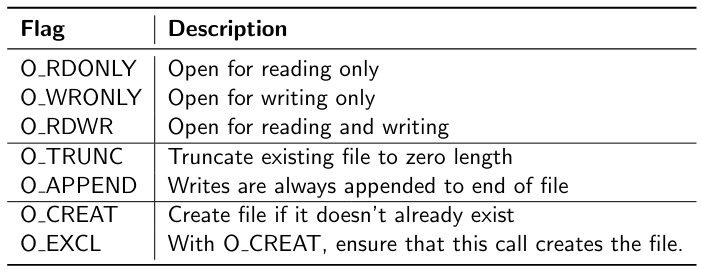
\includegraphics[width=0.5\textwidth]{flag_open.png}
    \end{center}
    Tabella delle mode disponibili:
    \begin{center}
        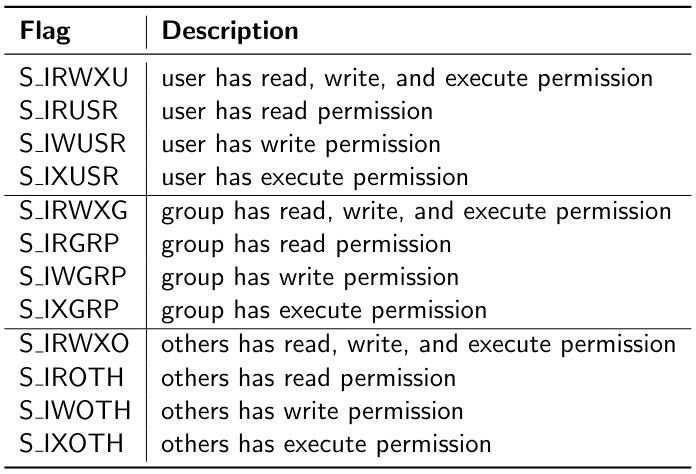
\includegraphics[width=0.5\textwidth]{mode_open.png}
    \end{center}
    Se non vengono forniti i permessi cosa succederà al file?
    All'interno del SO esiste la \verb|umask| con dei valori che 
    di default non dà permessi allo user e solo scrittura
    a group e others, tale valore sarà 022. Di \verb|umask|
    ne esiste una sola, andando a fornire dei permessi tramite 
    la \verb|open| i permessi che il file avrà saranno 
    la \verb|mode| con il negato della \verb|umask| (mode and
    $\sim$umask. 
    Vari esempi di utilizzo:
    \begin{lstlisting}[language=C]
        int fd;
        //Open existing file for only writing
        fd = open("myfile", O_WRONLY);

        //Open new or existing file for reading/writing, truncating 
        // to zero bytes; file permissions read+write only for owner
        fd = open("myfile", O_RDWR | O_CREAT | O_TRUNC, S_IRUSR | S_IWUSR);
    \end{lstlisting}
    
    \subsection{read}

    Prende in input il file descriptor ottenuto tramite la 
     \verb|open|, un \verb|buffer| dove andremo a salvare quello che 
    leggeremo dal file e un \verb|size_t| che definisce il numero di byte 
    che vogliamo leggere dal file. In caso di successo ritornerà 
    un valore \verb|ssize_t| che dovrebbe essere uguale o minore a \verb|count|, in caso di
    errore tornerà un -1.
    \begin{lstlisting}[language=C]
        #include <stdio.h> 

        //Returns number of bytes read, or -1 on error
        ssize_t read(int fd, void *buf, size_t count);
    \end{lstlisting}
    Esempio d'uso:
    \begin{lstlisting}[language=C]
        //Open existing file for reading
        int fd = open("myfile", O_RDONLY);
        if(fd == -1)
            errExit("open");
        
        // A MAX_READ bytes buffer
        char buffer[MAX_READ + 1];

        //Reading up to MAX_READ bytes from myfile
        ssize_t numRead = read(fd, buffer, MAX_READ);
        if(numRead == -1)
            errExit("Read");
    \end{lstlisting}
    Un esempio di lettura da Standard Input:
    \begin{lstlisting}[language=C]
        // A MAX_READ bytes buffer
        char buffer[MAX_READ + 1];

        //Reading up to MAX_READ bytes from STDIN
        ssize_t numRead = read(STDIN_FILENO, buffer, MAX_READ);
        if(numRead == -1)
            errExit("read");
        
        buffer[numRead] = '\0';
        printf("Input data: %s\n", buffer);
    \end{lstlisting}

    \subsection{write}

    Ci permette di scrivere su un file descriptor
    \begin{lstlisting}[language=C]
        #include <unistd.h>

        //Returns number of bytes written, or -1 on error
        sszie_t write(int fd, void *buf, size_t count);
    \end{lstlisting}
    Esempio di scrittura:
    \begin{lstlisting}[language=C]
        //Open existing file fro writing
        int fd = open("myfile", O_WRONLY);
        int(fd == -1)
            errExit("open");

        //A buffer collecting the string
        char buffer[] = "Ciao Mondo";

        //Writing up to sizeof(buffer) bytes into myfile
        ssize_t numWrite = write(fd, buffer, sizeof(buffer));
        if(numWrite != sizeof(buffer))
            errExit("write");
    \end{lstlisting}
    Per scrivere su terminale, come prima si userà \verb|STDOUT_FILENO| al posto del file descriptor.

    \subsection{lseek}

    Una volta aperto un file, il kernel salva un file offset
    ovvero un indicatore di un valore che identifica a quale punto 
    di scrittura/lettura siamo arrivati. Per utilizzare tale 
    cursore useremo la \verb|lseek|.
    \begin{lstlisting}[language=C]
        #include <unistd.h>

        //Returns the resulting offset location, or -1 on error
        off_t write(int fd, off_t offset, int whence);
    \end{lstlisting}
    \begin{description}
        \item[N.B.:] \verb|whence| indica la base di partenza dell'offset; 
    \end{description}
    Esempio di utilizzo:
    \begin{lstlisting}[language=C]
        #include <unistd.h>

        //Returns number of bytes written, or -1 on error
        sszie_t write(int fd, void *buf, size_t count);
    \end{lstlisting}
    Alcuni esempi:
    \begin{lstlisting}[language=C]
        //first byte of the file
        off_t current = lseek(fd1, 0, SEEK_SET);
        //last byte of the file
        off_t current = lseek(fd2, -1, SEEK_END);
        //10th byte past the current offset location of the file
        off_t current = lseek(fd3, -10, SEEK_CUR);
        //10th byte after the current offset location of the file
        off_t current = lseek(fd4, 10, SEEK_CUR);
    \end{lstlisting}
    \begin{center}
        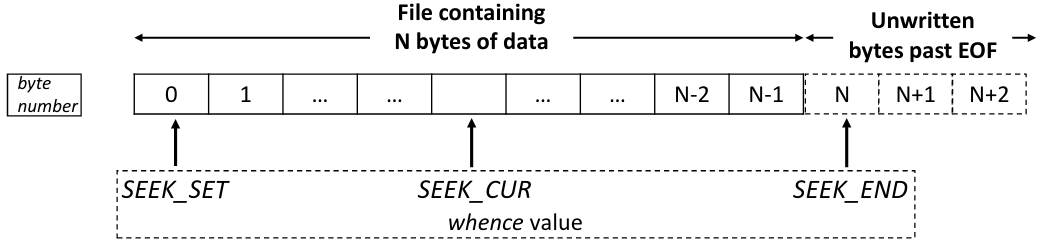
\includegraphics[width=0.5\textwidth]{lseek.png}
    \end{center}

    \subsection{close}

    \begin{lstlisting}[language=C]
        #include <unistd.h>

        //Returns 0 on success, or -1 on error
        int close(int fd);
    \end{lstlisting}
    Tutti i file descriptor vengono chiusi quando un processo 
    termina, ma è buona prassi chiudere sempre. La chiusura 
    \textbf{non} elimina il file. 

    \subsection{unlink}

    \begin{lstlisting}[language=C]
        #include <unistd.h>

        //Returns 0 on success, or -1 on error
        it unlink(const char *pathname);
    \end{lstlisting}
    Prende in input il nome del file, perché il file descriptor
    può anche essere chiuso, se il file non ha altri symbolic 
    link, viene rimosso.
    \begin{description}
        \item[Symbolic link:] il collegamento su desktop, oppure il file è aperto da altri processi. 
    \end{description}
    \verb|unlink| \textbf{non} può rimuovere directory.

    \subsection{stat, lstat, fstat}

    \begin{lstlisting}[language=C]
        #include <sys/stat.h>

        //Returns 0 on success, or -1 on error
        int stat(const char *pathname, struct stat *statbuf);
        int lstat(const char *pathname, struct stat *statbuf);
        int fstat(int fd, struct stat *statbuf);
    \end{lstlisting}
    In caso di succeso la \verb|struct stat| viene popolata da 
    varie informazioni. La differenza tra queste system call 
    sono: 
    \begin{itemize}
        \item \verb|stat| ritorna informazioni relative a un file tramite il nome o path;
        \item \verb|lstat| se \verb|pathname| è un symbolic link, ritornerà le informazioni sul link stesso e non sul file a cui punta;
        \item \verb|fstat| utilizza il file descriptor;
    \end{itemize}
    
    \subsection{Mode}

    Si tratta di una bit mask, presente anche nella \verb|struct stat|
    , che ci permette di definire i permessi dei file. 
    Lunga 16 bit, i primi 9 sono per other, group e user, 
    rispettivamente 3 a testa. Possiamo usarla per avere 
    informazioni sulla tipologia del file. Esempio:
    \begin{lstlisting}[language=C]
        char pathname[] = "/tmp/file.txt";
        struct stat statbuf;
        //Getting the attribute of /tmp/file.txt
        if(stat(pathname, &statbuf) == -1)
            errExit("stat");

        //Checking if /tmp/file.txt is a regular file
        if((statbuf.st_mode & S_IFMT) == S_IFREG)
            printf("regular file!\n);

        //Equivalently, checking if /tmp/file.txt is a 
        //regular file by S_ISREG macro
        if(S_ISREG(statbuf.st_mode))
            printf("regular file!\n");
    \end{lstlisting}
    \begin{center}
        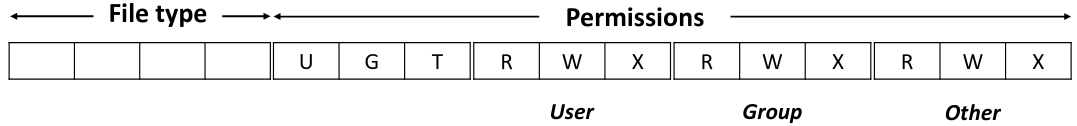
\includegraphics[width=0.5\textwidth]{st_mode.png}
    \end{center}
    I bit oltre i 9 dedicati a other, group e user hanno 
    i seguenti significati:
    \begin{itemize}
        \item U identifica se l'utente che sta eseguendo quell'eseguibile è lo stesso utente proprietario dell'eseguibile;
        \item G verifica se il gruppo che sta eseguendo è il gruppo proprietario;
        \item T è lo sticky bit, funziona come un bit che non ci permette di cancellare quel file;
    \end{itemize}
    File e directory sono la stessa cosa, per modificare i permessi 
    di una directory si usano le stesse mode dei file.

    \subsection{access}

    Controlla l'accessibilità di un file relativamento 
    al nostro user id e group id.
    \begin{lstlisting}[language=C]
        #include <unistd.h>

        //Returns 0 if all permissions are granted, otherwise -1
        int access(const char *pathname, int mode)
    \end{lstlisting}
    Le possibili mode che si possono usare insieme 
    a questa system call sono queste:
    \begin{center}
        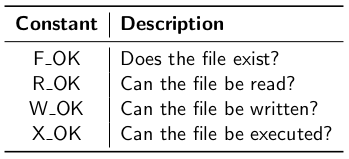
\includegraphics[width=0.5\textwidth]{access.png}
    \end{center}

    \subsection{chmod e fchmod}

    Permettono di cambiare i permessi di un file prendendo
    in input il pathname o il file descriptor più le eventuali
    \verb|mode| di interesse.
    \begin{lstlisting}[language=C]
        //All return 0 on success, or -1 on error
        #include <sys/stat.h>

        int chmod(const char *pathname, mode_t mode);

        #define _BSD_SOURCE
        #include <sys/stat.h>

        int fchmod(int fd, mode_t mode);
    \end{lstlisting}

    \section{Directory}

    \subsection{mkdir}

    Prende in input il \verb|pathname| della directory e 
    una \verb|mode|.
    \begin{lstlisting}[language=C]
        #include <sys/stat.h>

        //Returns 0 on success, or -1 on error.
        int mkdir(const char *pathname, mode_t mode);
    \end{lstlisting}
    I parametri mode sono gli stessi della \verb|open|,
    se la directory esistesse già, il valore di ritorno sarà 
    sempre -1, ma la variabile \verb|errno| conterrà 
    il messaggio \verb|EEXIST|, a indicare che tale 
    directory è già presente.

    \subsection{rmdir}

    \begin{lstlisting}[language=C]
        #include <unistd.h>

        //Returns 0 on success, or -1 on error.
        int rmdir(const char *pathname);
    \end{lstlisting}
    Se esiste anche un solo file all'interno dello directory
    tale system call tornerà -1 di errore, per avere successso
    deve essere completamente vuota.

    \subsection{opendir, closedir e readdir}

    \begin{lstlisting}[language=C]
        #include <sys/types.h>
        #include <dirent.h>

        //Returns directory stream handler, or NULL on error.
        DIR *opendir(const char *dirpath);

        //Returns 0 on success, or -1 on error
        int closedir(DIR *dirp);
    \end{lstlisting}
    Una volta aperta una directory per leggerla si userà
    \begin{lstlisting}[language=C]
        #include <sys/types.h>
        #include <dirent.h>

        //Returns pointer to an allocated structure describing the
        //next directory entry or NULL on end-of-directory or error
        struct dirent *readdir(DIR *dirp);
    \end{lstlisting}
    La struttura di riferimento per la \verb|readdir|:
    \begin{center}
        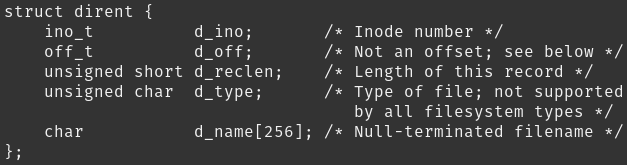
\includegraphics[width=0.5\textwidth]{dirent.png}
    \end{center}
    Tramite il \verb|d_type| possiamo ottenere delle informazioni
    sul tipo di file che stiamo scorrendo:
    \begin{center}
        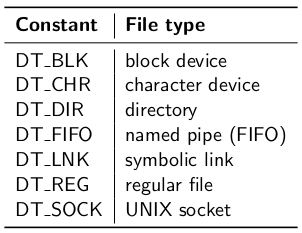
\includegraphics[width=0.5\textwidth]{d_type.png}
    \end{center}
    Esempio d'uso:
    \begin{lstlisting}[language=C]
        DIR *dp = opendir("myDir");
        if(dp == NULL)
            return -1;
        
        errno = 0;
        struct dirent *dentry;
        //Iterate until NULL is returned as a result
        while((dentry = readdir(dp)) != NULL){
            if(dentry->d_type == DT_REG)
                printf("Regular file: %s\n", dentry->d_name);
            errno = 0;
        }
        //NULL is returned on error, and when the end-of-directory is reached!
        if(errno != 0)
        printf("Error while reading dir.\n");
        closedir(dp);
    \end{lstlisting}

    \chapter{Processi}

    \section{Identificatori}

    Ogni processo è caratterizzato da un PID univoco che cambia 
    sempre, l'unico processo a mantenere sempre lo stesso 
    identificatore è il processo \verb|INIT|.

    \subsection{getpid}

    \begin{lstlisting}[language=C]
        #include <unistd.h>
        #include <sys/types.h>

        pid_t getpid(void);
    \end{lstlisting}
    Ritorna come valore il PID del processo chiamante e \textbf{non può
    fallire}.

    \subsection{getuid, geteuid, getgid e getegid}

    Anche queste system call \textbf{hanno sempre successo}.
    La differenza \verb|getuid| e \verb|geteuid|, ovvero
    tra real user ed effective user, consiste che il 
    real user (vale anche per il real group), identificano 
    l'utente o il gruppo a cui appartiene il processo, 
    mentre l'effective è quello che viene usato dal SO, 
    per gestire operazioni solitamente non permesse (come 
    installare tramite packet manager, si usa \verb|sudo|). 

    \section{Environment}

    Ad ogni processo viene associato un array \verb|environ|,
    di stringhe che contiene tutte le variabili di
    ambiente salvate all'interno di \verb|environ|

    Esempio:
    \begin{lstlisting}[language=C]
        #include <stdio.h>
        //Global variable pointing to the environment of the process
        extern char **environ;

        int main(int argc, char *argv[]){
            for(char **it = environ; (*it) != NULL; ++it){
                printf("--> %s\n", *it);
            }
            return 0;
        }
    \end{lstlisting}  
    
    \subsection{getenv, setenv, unsetenv}

    \begin{lstlisting}[language=C]
        #include <stlib.h>
        //Returns pointer to (value) string, or NULL if no such variable exists
        char *getenv(const char *name);
        //Returns 0 on success, or -1 on error
        int setenv(const char *name, const char *value, int overwrite);
        //Returns 0 on success, or -1 on error
        int unsetenv(const char *name);
    \end{lstlisting} 
    Sono system call che interagiscono con l'environment.
    \verb|setenv| aggiunge la variabile \verb|name| all'environment 
    con il valore \verb|value|, se \verb|name| non esiste. Nel caso 
    in cui \verb|name| esistesse, allora il suo valore verrebbe 
    cambiato in \verb|value| se \verb|overwrite| è diverso da 0, se fosse 
    uguale a 0 il valore non verrebbe modificato, ma comunque 
    \verb|setenv| avrebbe successo.

    \section{Working directory}

    \subsection{getcwd}

    Per identificare la directory in cui io sto lavorando
    in questo momento, si usa la system call \verb|getcwd|
    \begin{lstlisting}[language=C]
        #include <unistd.h>

        //Returns cwdbuf on success, or NULL on error
        char *getcwd(char *cwdbuf, size_t size);
    \end{lstlisting} 
    Ritorna \verb|NULL| nell'eventualità che il pathname 
    sia più lungo della \verb|size| data, oppure ritorna 
    il pathname assoluto dell'attuale working directory.

    \subsection{chdir, fchdir}

    L'attuale working directory viene usata per interpretare 
    i path relativi.

    \begin{lstlisting}[language=C]
        #include <unistd.h>

        //Returns 0 on success, or -1 on error
        int chdir(const char *pathname);
    \end{lstlisting} 
    Permette di cambiare la directory attuale tramite 
    l'uso del pathname.

    \begin{lstlisting}[language=C]
        #define _BSD_SOURCE
        #include <unistd.h>

        //Returns 0 on success, or -1 on error
        int fchdir(int fd);
    \end{lstlisting} 
    Permette di cambiare la directory attuale tramite 
    l'uso del file descriptor.

    \section{File descriptor table}

    Per visualizzare la file descriptor table di un processo
    basta andare all'interno della cartella 
    \verb|/proc/<PID>/fd|, dove \verb|fd| è un symbolic 
    link per ogni riga della tabella. Si potranno trovare 
    anche socket e pipe.
    
    \subsection{dup}

    \begin{lstlisting}[language=C]
        #include <unistd.h>

        //Returns (new) file descriptor on success, or -1 on error
        int dup(int oldfd);
    \end{lstlisting} 
    Ritornerà un nuovo file descriptor a partire da uno 
    che si ha già, ovviamente partendo dal valore più basso
    disponibile, potranno essere usati entrambi intercambiabilmente.

    \section{Operazioni con i processi}

    \subsection{exit, atexit}

    \begin{lstlisting}[language=C]
        #include <stdlib.h>

        void exit(int status);
    \end{lstlisting} 
    Al suo interno chiama un'altra system call \verb|_exit|,
    va \textbf{sempre} a buon fine. La terminazione 
    del processo può essere gestita da noi tramite
    \verb|atexit|
    
    \begin{lstlisting}[language=C]
        #include <stdlib.h> 
        //Returns 0 on success, or nonzero on error

        int atexit(void (*func)(void));
    \end{lstlisting} 
    Il puntatore a funzione preso come parametro, quando 
    viene creato non va a finire all'interno del layout 
    di memoria del processo.

    Esempio pratico
    \begin{lstlisting}[language=C]
        #include <stdio.h>
        #include <stdlib.h>
        #include <unistd.h>

        void func1(){
            printf("\tAtexit function 1 called\n");
        }
        void func2(){
            printf("\tAtexit function 2 called\n");
        }

        int main(int argc, char *argv[]){
            if(atexit(func1) != 0 || atexit(func2) != 0)
                _exit(EXIT_FAILURE);
            exit(EXIT:SUCCESS);
        }
    \end{lstlisting}
    L'eventuala output sarà
    \begin{lstlisting}[language=C]
        Atexit function 2 called
        Atexit function 1 called
    \end{lstlisting}
    Eseguire un \verb|return(n)| è equivalente all'eseguire 
    un \verb|exit(n)|, se il \verb|return| non viene messo il 
    programma metterà in automatico il \verb|return(0)|.

    \section{Creazione dei processi}

    \subsection{fork}

    \begin{lstlisting}[language=C]
        #include <unistd.h>

        //In parent: returns process ID of child on success, or -1 on error
        //In created child: always returns 0
        pid_t fork(void);
    \end{lstlisting}
    Il processo figlio sarà una copia del padre in tutto e per tutto e inizieranno 
    a eseguire in parallelo, ovviamente l'esecuzione non è sincrona. L'unica differenza tra 
    i due è la variabile di ritorno \verb|pid_t| che sarà 0 per il figlio, mentre per il 
    padre conterrà il PID del figlio. Si userà il valore 0 per far fare delle operazioni 
    specifiche esclusivamente al figlio magari. 

    Il figlio eredita tutto quello che il padre aveva già aperto, istanziato, etc.
    Esempio:
    \begin{lstlisting}[language=C]
        #include <unistd.h>
        
        int main(){
            int stack = 111;
            pid_t pid = fork();
            if(pid == -1)
                errExit("fork");
            //Both parent and child come here 
            if(pid == 0)
                stack = stack *4;
            printf("\t%s stack %d\n", (pid == 0) ? "(child)" : "(parent)", stack);
        }
    \end{lstlisting}
    
    \subsection{getppid}

    Permette di ottenere il pid del padre.
    \begin{lstlisting}[language=C]
        #include <unistd.h>

        //Always succesfully returns PID of caller's parent 
        pid_t getppid(void);
    \end{lstlisting}
    Torna sempre il PID del padre di norma, ma se dovesse succedere 
    che il padre termini prima del figlio, in quel caso tornerà il PID del 
    processo che ha ereditato il figlio, di normale tale processo è \verb|INIT| 
    ovvero il processo con PID 1.

    \section{Monitoring}

    I metodi del padre per monitorare i figli 

    \subsection{wait}

    \begin{lstlisting}[language=C]
        #include <sys/wait.h>

        //Returns PID of terminated child, or -1 on error 
        pid_t wait(int *status);
    \end{lstlisting}
    Prende in input uno status o anche \verb|NULL|, con \verb|NULL| come 
    status, il padre aspetterà la terminazione di uno qualunque dei suoi 
    figli. Questa system call blocca il padre.

    Se un padre che non ha più figli, fa la \verb|wait| gli ritornerà 
    un -1, ma per capire che non ci sono più figli ovviamente 
    dobbiamo guardare il contenuto della variabile \verb|errno|
    che in questa casistica conterrà \verb|ECHILD|.

    Se si volesse aspettare tutti i figli occorrerà mettere questa 
    chiamata in un ciclo \verb|while|, se status non è \verb|NULL|
    la system call darà come ritorno gli stati di terminazione del figlio 
    come \verb|exit(1)| o \verb|exit(0)|.

    \subsection{waitpid}

    La differenza con la \verb|wait| è che questa aspetta un figlio 
    specifico in base al valore del PID
    \begin{lstlisting}[language=C]
        #include <sys/wait.h>

        //Returns a PID, 0 or -1 on error
        pid_t waitpid(pid_t pid, int *status, int options);
    \end{lstlisting}
    In base al valore inserito in \verb|pid| si comporta diversamente:
    \begin{itemize}
        \item \verb|pid| $\ge$ 0, aspetta il figlio con quello specifico PID;
        \item \verb|pid| = 0, aspetta la terminazione di ogni figlio nello stesso process group(originati tutti dallo stesso padre);
        \item \verb|pid| < -1, aspetta che uno dei processi del process group con quel PID passato, termini;
        \item \verb|pid| = -1, aspetta un qualsiasi processo termini.
    \end{itemize}
    Per le options si possono usare:
    \begin{description}
        \item[WUNTRACED]: ritorna il PID del figlio sia quando viene terminato che quando viene stoppato;
        \item[WCONTINUED]: ritorna quando un figlio è stato rimesso in esecuzione dopo essere stato stoppato;
        \item[WNOHANG]: non è bloccante, quindi fino a quando i figli indicati dal pid non hanno cambiato status, il padre che la chiama continuerà a fare altro, in questo caso il valore di ritorno della \verb|waitpid| è 0;
        \item[0]: aspetta solo per i figli che terminano.    
    \end{description}
    \begin{lstlisting}[language=C]
        pid_t pid;
        for(int i = 0; i < 3; ++i){
            pid = fork();
            if(pid == 0){
                //Code executed by the child process... 
                exit(0);
            }
        }
        //The parent process only waits for the last created child 
        waitpid(pid, NULL, 0);
    \end{lstlisting}
    Altro esempio:
    \begin{lstlisting}[language=C]
        pid_t pid = fork();
        if(pid == 0){
            //Code executed by the child process
        }
        else{
            //Waiting for a terminated/stopped | resumed child process 
            waitpid(pid, NULL, WUNTRACED | WCONTINUED);
        }
    \end{lstlisting}
    Lo status è un intero a 16 bit, gli 8 bit più significativi vengono 
    usati per capire lo status di uscita(quindi i possibili valori vanno da 0 a 255).
    Inoltre vengono fornite dal SO delle macro per capire come il processo figlio ha 
    terminato 
    \begin{description}
        \item[WIFEXITED]: ritorna true se il figlio termina normalmente;
        \item[WEXITSTATUS]: ritorna lo status con cui ha terminato il processo figlio;
        \item[WIFSIGNALED]: ritorna true se il processo figlio è stato ucciso con un segnale;
        \item[WTERMSIG]: ritorna il numero del segnale che ha causato la terminazione del figlio;
        \item[WIFSTOPPED]:   ritorna true se il processo è stato stoppato con un segnale;
        \item[WSTOPSIG]: ritorna il numero del segnale che stoppato il processo figlio;
        \item[WIFCONTINUED]: ritorna true se il figlio ha ripreso l'esecuzione tramite un \verb|SIGCONT|.         
    \end{description}
    Esempi vari:
    \begin{lstlisting}[language=C]
        waitpid(-1, &status, WUNTRACED | WCONTINUED);
        if(WIFEXITED(status)){
            printf("Child exited, status = %s\n", WEXITSTATUS(status));
        }
    \end{lstlisting}
    \begin{lstlisting}[language=C]
        waitpid(-1, &status, WUNTRACED | WCONTINUED);
        if(WIFSIGNALED(status)){
            printf("child killed by signal %d (%s)", WTERMSIG(status), strsignal(WTERMSIG(status)));
        }
    \end{lstlisting}

    \section{Program execution}

    \subsection{exec system calls}

    La system call \verb|exec|, non crea figli, un processo che chiama 
    tale system call viene rimodellato, prende l'eseguibile a cui punta 
    e lo rimappa all'interno del processo chiamante. Trasforma tutto il contenuto del
    processo chiamante, il PID \textbf{non} cambia.
    \begin{lstlisting}[language=C]
        #include <unistd.h>
        //None of the following returns on success, all return -1 on error 
        int execl(const char *path, const char *arg, ...); //variadic functions
        int execlp(const char *path, const char *arg, ...);
        int execle(const char *path, const char *arg, ..., char *const envp[]);
        int execv(const char *path, char *const argv[]);
        int execvp(const char *path, char *const argv[]);
        int execve(const char *path, char *const argv[], char *const envp[]);
    \end{lstlisting}
    L'ultimo parametro delle \verb|execl| deve essere sempre un \verb|NULL|.
    \begin{center}
        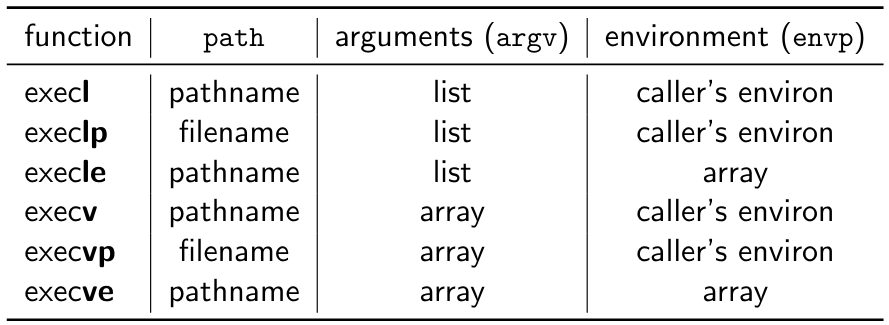
\includegraphics[width=0.5\textwidth]{exec.png}
    \end{center}
    \begin{description}
        \item[path]: per pathname ci si riferisce al path assoluto all'eseguibile,
        mentre con filename al nome dell'eseguibile che si deve trovare nella lista 
        delle directory del PATH environ;
        \item[argv]: una lista o array terminata da \verb|NULL|, che definiscono gli argomenti del programma;
        \item[envp]: un array di puntatori a stringhe terminato da \verb|NULL| che definiscono l'environ del programma.  
    \end{description}
    Esempio:
    \begin{lstlisting}[language=C]
        #include <stdio.h>
        #include <unistd.h>
        #include <stdlib.h>
        
        int main(int argc, char *argv[]){
            printf("PID of example.c = %d\n", getpid());
            char *args[] = {"Hello.c", "C", "Programming", NULL};
            execv("./hello", args);
            printf("Back to example.c");

            return 0;
        }
    \end{lstlisting}
    Eseguendo sia questo codice che "Hello.c" il primo programma 
    andrà a essere rimodellato con il codice all'interno di "Hello.c".

    \chapter{Interprocess communication}

    Sono dei meccanismi utilizzati per coordinare/sincronizzare attività 
    tra vari processi. Di base le IPC possono essere create tramite 
    un comando con \verb|get|, prendono come primo parametro 
    una chiave che serve ai processi per poter comunicare 
    tra di loro, senza non riuscirebbero. Ognuna di queste 
    ritorna un file descriptor.

    \section{Creazione delle chavi}

    Le chiavi delle system V IPC, sono dei tipi \verb|key_t|
    e praticamente sono degli \verb|int|, possono essere definite 
    da noi o lasciare che si arrangi il SO. Una chiave è univoca 
    un'eventuale creazione di due IPC differenti con la stessa 
    chiave porterebbe a una sovrascrizione. Per delegarne 
    la creazione al SO si utilizza la macro \verb|IPC_PRIVATE|, 
    che in automatico genera una chiave univoca verificando 
    prima le chiavi già in uso.

    Un'altra modalità è tramite l'uso della system call 
    \verb|ftok| 
    \begin{lstlisting}[language=C]
        #include <sys/ipc.h>

        //Returns integer key on success, or -1 on error(check errno)
        key_t ftok(char *pathname, int proj_id);
    \end{lstlisting}
    Il \verb|proj_id| può essere un qualunque \verb|int| 
    l'importante che i suoi ultimi 8 bit siano diversi da 0
    visto che saranno quelli che verranno usati per la creazione, 
    usando dei caratteri ASCII si ha la certezza che gli 
    ultimi 8 bit non saranno uguali a 0.
    
    Un ultimo possibile metodo è definirle manualmente, con 
    il rischio di usare chiavi già in uso.

    \section{Data Structure}

    Ogni IPC ha una sua struttura, ma ognuna ne ha una in comune,
    ovvero la struttura \verb|ipc_perm|:
    \begin{lstlisting}[language=C]
        struct ipc_perm{
            key_t __key;            //Key, as supplied to 'get' call
            uid_t uid;              //Owner's user ID
            gid_t gid;              //Owner's group ID
            uid_t cuid;             //Creator's user ID
            gid_t cgid;             //Creator's group ID
            unsigned short mode;    //Permissions
            unsigned short __seq;    //Sequence number
        }
    \end{lstlisting}
    Le \verb|mode| sono una serie di permessi che possono 
    essere settati. \verb|cuid| e \verb|gid| sono immutabili.
    Inoltre le IPC possono avere solo permessi di lettura 
    e scrittura, non di esecuzione.
    Esempio:
    \begin{lstlisting}[language=C]
        struct semid_ds semq;
        //get the data structure of a semaphore from the kernel 
        if(semctl(semid, 0, IPC_STAT, &semq) == -1)
            errExit("semctl get failed");
        //change the owner of the semaphore
        semq.sem_perm.uid = newuid;
        //update the kernel copy of the data structure 
        if(semctl(semid, IPC_SET, &semq) == -1)
            errExit("semctl set failed");
    \end{lstlisting}
    
    \section{IPC commands}

    \subsection{ipcs}

    \verb|ipcs| da terminale, mostra tutti i dettagli 
    delle IPC esistenti in quell'istante all'interno del SO.
    Tali dettagli sono:
    \begin{itemize}
        \item key;
        \item owner;
        \item permessi;
        \item dimensione;
    \end{itemize}
    Più altri dettagli specifici per la singola IPC.
    
    \subsection{ipcrm}

    \verb|ipcrm| permette di eliminare delle IPC che sono 
    ancora attive, nel caso in cui non venga gestita la cosa 
    dal programmatore.

    \section{Semaphores}

    \subsection{semget}

    \verb|semget| è la system call che permette di creare 
    un set di semafori.
    \begin{lstlisting}[language=C]
        #include <sys/sem.h>

        //Returns semaphore set identifier on success, or -1 on error 
        int semget(key_t key, int nsems, int semflg);
    \end{lstlisting}
    Prende come parametri una chiave, un numero di semafori 
    che dovrà essere contenuto dal set di semafori e infine 
     delle flag. Tali flag possono essere 
    una qualsiasi della \verb|open| (non i permessi di 
    esecuzione siccome le IPC non ne necessitano), in aggiunta 
    si metteranno sempre in or \verb|IPC_CREAT| e la 
    \verb|IPC_EXCL|, che differenza c'è tra queste due flag? 
    La prima dice che se il semaforo con quella chiave non 
    esiste lo crea, nel caso in cui esista, restituisce 
    l'ID di quel set di semafori. La seconda insieme alla prima
    farà fallire la system call in caso la chiave in input sia 
    già in uso per un altro set di semafori. Questo è comodo 
    in base al fatto che si voglia creare un set di semafori nuovo 
    oppure ottenere l'ID di un set esistente.

    \subsection{semctl}

    Permette di svolgere svariate operazioni su un determinato 
    set di semafori.
    \begin{lstlisting}[language=C]
        #include <sys/sem.h>

        //Returns non negative integer on success, or -1 on error 
        int semctl(int semid, int semnum, int cmd, .../*union semnum arg*/);
    \end{lstlisting}
    \verb|semid| è l'identificatore del set di semafori, su 
    cui le operazioni verranno effettuate. \verb|semnum|
    è un identificatore specifico per un semaforo all'interno del 
    set, mettendo 0 si agirà sull'intero set in base all'eventuale \verb|cmd|
    passata.
    \verb|cmd| possono essere una serie di flag. Infine si passerà 
    una \verb|union|,
    funziona in maniera simile a una \verb|struct|, permette di definire al 
    suo interno vari campi, ma dal punto di vista del SO, 
    per quella \verb|union| verrà allocata una memoria pari alla 
    dimensione della variabile più grande al suo interno, adatta
    alle ottimizzazioni.

    Esempio:
    \begin{lstlisting}[language=C]
        #ifndef SEMUN_H
        #define SEMUN_H
        #include <sys/sem.h>
        //definition of the union semun 
        union semun{
            int val;                //per operazioni su singolo semaforo
            struct semid_ds *buf;   //su permessi 
            unsigned short *array;  //su un intero set di semafori
        };
        #endif
    \end{lstlisting}
    In questo caso verrà allocata memoria equivalente alla 
    \verb|struct semid_ds|.

    \subsubsection{Flag}

    \begin{lstlisting}[language=C]
        int semctl(semid, 0 /*ignored*/, cmd, arg);
    \end{lstlisting}
    L'elenco delle flag da usare con \verb|semctl| al parametro 
    \verb|cmd|
    \begin{itemize}
        \item \verb|IPC_RMID|: deve essere usata per eliminare l'IPC 
        alla fine del suo utilizzo;
        \item \verb|IPC_STAT|: permette di salvare lo stato dell'IPC 
        all'interno della \verb|strcut semid_ds|, verrà salvato 
        all'interno di \verb|arg.buf|;
        \item \verb|IPC_SET|: occore per settare i nuovi permessi
        passando in input \verb|arg| modificato;
    \end{itemize}
    \begin{lstlisting}[language=C]
        struct semid_ds{
            struct ipc_perm sem_perm; //ownership and permissions
            time_t sem_otime; //Time of last semop()
            time_t sem_ctime; //Time of last change
            unsigned long sem_nsems; //Number of semaphores in set
        };
    \end{lstlisting}
    Esempio di modifica dei permessi di un set di semafori:
    \begin{lstlisting}[language=C]
        int semid = semget(key, 10, IPC_CREAT | S_IRUSR | S_IWUSR);
        //instantiate a semid_ds struct 
        strcut semid_ds ds;
        //instantiate a semun union(defined manually somewhere)
        union semun arg;
        arg.buf = &ds;
        //get a copy of semid_ds structure belonging to the kernel 
        if(semctl(semid, 0 /*ignored*/, IPC_STAT, arg) == -1)
            errExit("semctl IPC_STAT failed");
        //update permissions to guarantee read access to the group 
        arg.buf->sem_perms.mode |= S_IRGRP;
        //update the semid_ds structure of the kernel 
        if(semctl(semid, 0 /*ignored*/, IPC_SET, arg) == -1)
            errExit("semctl IPC_SET failed");
    \end{lstlisting}

    \subsubsection{Semaphore Control Operations}

    \begin{lstlisting}[language=C]
        int semctl(semid, semnum, cmd, arg);
    \end{lstlisting}
    Per usare i \verb|cmd| \verb|SETVAL| e \verb|GETVAL|
    occorre specificare il semaforo singolo del set.
    \begin{itemize}
        \item \verb|SETVAL| si usa il campo val della 
        union e si setta il singolo semaforo a quel 
        valore;
        \item \verb|GETVAL| ritorna il valore del 
        semaforo in \verb|arg.val|.
    \end{itemize}
    Se invece si vuole lavorare con l'intero set di semafori si userà 0 
    come \verb|semnum|:
    \begin{lstlisting}[language=C]
        int semctl(semid, 0 /*ignored*/, cmd, arg);
    \end{lstlisting}
    \begin{itemize}
        \item \verb|SETALL| si usa il campo array della 
        \verb|union| e si setta l'intero set del semaforo
        con quei valori;
        \item \verb|GETALL| salva in \verb|arg.array| tutti 
        i valori dei semafori.
    \end{itemize}
    Esempio per settare i valori di un set:
    \begin{lstlisting}[language=C]
        int semid = semget(key, 10, IPC_CREAT | S_IRUSR | S_IWUSR);
        //set the first 5 semaphores to 1, and the remaining to 0
        int values[] = {1, 1, 1, 1, 1, 0, 0, 0, 0, 0};
        union semun arg;
        arg.array = values;
        //initialize the semaphore set 
        if(semctl(semid, 0/*ignored*/, SETALL, arg) == -1)
            errExit("semctl SETALL");
    \end{lstlisting}
    Altre operazioni:
    \begin{lstlisting}[language=C]
        int semctl(semid, semnum, cmd, 0);
    \end{lstlisting}
    \begin{itemize}
        \item \verb|GETPID|: ritorna il PID dell'ultimo 
        processo che ha fatto una semop sul semaforo specificato;
        \item \verb|GETNCNT|: ritorna il numero dei processi 
        in attesa che il valore di un semaforo diventi positivo;
        \item \verb|GETZCNT|: ritorna il numero di processi che 
        attualmente stanno aspettando che un semaforo diventi 
        zero.
    \end{itemize}
    
    \subsection{semop}

    \begin{lstlisting}[language=C]
        #include <sys/sem.h>

        //Returns 0 on success, or -1 on error 
        int semop(int semid, struct sembuf *sops, unsigned int nsops);
    \end{lstlisting}
    La struttura \verb|sembuf| è la seguente:
    \begin{lstlisting}[language=C]
        struct sembuf{
            unsigned shor sem_num; //semaphore number 
            short sem_op; //operation to be performed 
            short sem_flag; //operation flags
        }
    \end{lstlisting}
    \verb|nsops| indica la dimensione della \verb|struct|,
    sono tutte operazioni a livello atomico. Se \verb|sem_op| 
    è positiva, si va ad aggiungere tale valore al semaforo 
    in oggetto, di conseguenza se negativa avverrà una 
    differenza. Invece se \verb|sem_op| è uguale a 0 e il
    semaforo è positivo, il processo che chiama rimarrà
    bloccato fino a quando il semaforo non sarà uguale a 0.
    
    Usando la \verb|sem_flag| \verb|IPC_NOWAIT|, la chiamata 
    non sarà bloccante e tornerà un errore \verb|EAGAIN|.

    Se il set di semafori viene rimosso, tutti i processi 
    bloccati vengono risvegliati e avranno in outpu \verb|EINTR|
    a indicare che lo sblocco è avvenuto per l'eliminazione 
    del semaforo.

    \section{Signals}

    Un segnale è una notifica a un processo che qualcosa 
    è avvenuto, un processo riceve un segnale nel momento 
    in cui avviene un certo evento o un altro processo 
    invia un segnale a un secondo processo. Durante il tempo 
    che passa tra la generazione del segnale e la ricezione
    si dice che il segnale è \textbf{pendente}. Normalmente 
    un segnale pendente raggiunge il processo target nell'istante 
    immediato in cui il target riottiene la possibilità 
    di usare la CPU, nel caso in cui la stesse già utilizzando 
    il segnale verrà ricevuto pressochè istantaneamente.
    Una volta ricevuto un segnale il processo destinatario 
    a seconda del segnale ricevuto:
    \begin{itemize}
        \item terminerà;
        \item si sospenderà/bloccherà;
        \item verrà ripreso dopo essere stato bloccato;
        \item il segnale verrà ignorato, quindi scartato dal kernel senza alcun effetto sul processo;
        \item il processo eseguirà un \verb|signal handler|, una funzione definita dal programmatore che esegue determinate azioni in base al segnale ricevuto.
    \end{itemize} 

    \subsection{Segnali di default}

    \subsubsection{Segnali per terminare un processo}

    \begin{description}
        \item[SIGTERM]: permette di terminare un processo, può essere gestito per lasciare il sistema in uno stato "safe";
        \item[SIGINT]: viene inviato a un processo quando si fa CTRL+C, anche questo è gestibile;
        \item[SIGQUIT]: usato per generare dei core dump e fare debug;
        \item[SIGKILL]: immediato, non è gestibile e termina il processo; 
    \end{description}

    \subsubsection{Segnali per bloccare e riprendere}

    \begin{description}
        \item[SIGSTOP]: blocca un processo immediatamente, non può essere bloccato, ignorato o gestito da un \verb|handler|;
        \item[SIGCONT]: fa riprendere l'esecuzione a un processo precedentemente bloccato.
    \end{description}

    \subsubsection{Altri segnali}

    \begin{description}
        \item[SIGPIPE]: generato quando un processo prova a scrivere su una PIPE o FIFO per le quali non c'è il corrispondente processo lettore;
        \item[SIGALRM]: segnale che usa un processo per mandare un segnale a sè stesso dopo un certo lasso di tempo;
        \item[SIGUSR1 e SIGUSR2]: vengono usati come più pare e piace da parte del programmatore.
    \end{description}

    \begin{center}
        \begin{tabular}{|c|c|c|c|}
            \hline 
            Nome & Numero & Può essere gestito? & Azione di default \\
            \hline 
            SIGTERM & 15 & si & termina un processo \\
            SIGINT & 2 & si & termina un processo \\
            SIGQUIT & 3 & si & core dump + terminazione \\
            SIGKILL & 9 & no & termina un processo \\
            SIGSTOP & 17 & no & blocca un processo \\
            SIGCONT & 19 & si & riprende un processo \\
            SIGPIPE & 13 & si & termina un processo \\
            SIGALRM & 14 & si & termina un processo \\
            SIGUSR1 & 30 & si & termina un processo \\
            SIGUSR2 & 31 & si & termina un processo \\
            \hline 
        \end{tabular}
    \end{center}

    Una tabella riassuntiva, la colonna "numero" indica 
    il codice per l'architettura x86 per inviare quel segnale 
    da terminale tramite il comando \verb|kill|.

    \subsection{signal handler}

    Un \verb|signal handler| è una funzione chiamata come 
    uno specifico segnale viene consegnato a un processo,
    la sua forma generale è la seguente:
    \begin{lstlisting}[language=C]
        void sigHandler(int sig){
            //code for the handler
        }
    \end{lstlisting}
    La funzione non ha alcun valore di ritorno, il paramentro 
    che prende è il segnale specifico. Quando il \verb|signal handler|
    è chiamato dal kernel, \verb|sig| è impostato con il 
    valore numerico del segnale consegnato al processo.

    Di base il SO ha un suo handler di default, che fa delle 
    operazioni sui dati di un processo che riceve un 
    \verb|SIGSTOP| o \verb|SIGKILL|.

    La chiamata a un \verb|signal handler| può interrompere 
    il flusso del programma principale in qualsiasi momento. 
    Il kernel invoca la funzione e una volta conclusa il
    programma riprende se può, da dove era stato interrotto.

    \subsection{signal}

    Una volta definito il \verb|signal handler| la system call
    \verb|signal| permette di settare quello definito 
    al posto di quello di default.

    \begin{lstlisting}[language=C]
        #include <signal.>

        typedef void (*signalhandler_t)(int);
        //Returns previous signal disposition on success, or SIG_ERR on error 
        sighandler_t signal(int signum, sighandler_t handler);
    \end{lstlisting}
    \verb|signum| identifica il segnale che voglia gestire, 
    mentre \verb|handler| può essere:
    \begin{itemize}
        \item l'indirizzo di un \verb|signal handler| definito dall'utente;
        \item la costante \verb|SIG_DFL| che resetta la disposizione di default del processo per il segnale \verb|signum|;
        \item la costante \verb|SIG_IGN| che setta il processo per ignorare la ricezione di una segnale \verb|signum|.
    \end{itemize}
    Esempio:
    \begin{lstlisting}[language=C]
        void sigHandler(int sig){
            printf("The signal %s was caught!\n",
             (sig == SIGINT) ? "CTRL-C" : "signal user-1");
        }
        int main(int argc. char *argv[]){
            //setting sigHandler to be executed for SIGINT or SIGUSR1
            if(signal(SIGINT, sigHandler) == SIG_ERR ||
            signal(SIGUSR1, sigHandler) == SIG_ERR){
                errExit("change signal handler failed");
            }
            //Do something else her. During this time, if SIGINT/SIGUSR1
            //is delivered, sigHandler will be used to handle the signal.
            //Reset the default process disposition for SIGINT and SIGUSR1
            if(signal(SIGINT, SIG_DFL) == SIG_ERR || 
            signal(SIGUSR1, SIG_DFL) == SIG_ERR){
                errExit("reset signal handler failed");
            }
            return 0;
        }
    \end{lstlisting}
    \begin{description}
        \item[N.B.:] la \verb|SIG_DFL| è una flag specifica per resettare.
    \end{description}
    Riassunto:
    \begin{itemize}
        \item \verb|SIGKILL| e \verb|SIGSTOP| non possono essere gestite;
        \item un segnale è un evento asincrono, non possiamo predire quando arriverà;
        \item quando viene chiamato un \verb|signal handler| il segnale che l'ha invocato viene automaticamente bloccato e sbloccato solo successivamente alla fine del \verb|signal handler|;
        \item se un segnale bloccato viene generato più volte, una volta sbloccato verrà consegnato al proccesso solo una;
        \item l'esecuzione di un \verb|signal handler| può essere interrotta da un segnale non bloccato;
        \item le disposizioni del segnale sono ereditate dai figli del processo padre.
    \end{itemize}

    \subsection{pause}

    \begin{lstlisting}[language=C]
        #include <unistd.h>
        //Always return -1 with errno set to EINTR
        int pause();
    \end{lstlisting}
    Sospende l'esecuzione del processo fino a quando un segnale 
    non viene catturato dal \verb|signal handler| o un 
    segnale non gestito lo termina.

    \subsection{sleep}

    \begin{lstlisting}[language=C]
        #include <unistd.h>
        unsigned int sleep(unsigned int seconds);
        /*Returns 0 on normal completion, or 
        number of unslept seconds if prematurely terminated*/
    \end{lstlisting}
    Sospende l'esecuzione del processo chiamante per un 
    numero specifico di secondi specificato nel parametro 
    \verb|seconds| o fino a quando un segnale non viene 
    catturato interrompendo la sospensione.

    \subsection{kill}

    \begin{lstlisting}[language=C]
        #include <signal.h>

        //Returns 0 on success, or -1 on error 
        int kill(pid_t pid, int sig);
    \end{lstlisting}
    Questa system call prende in input il PID del processo 
    a cui si vuole inviare il segnale e il tipo di segnale che 
    si vuole inviare. 
    \begin{itemize}
        \item (PID > 0): il segnale verrà inviato al processo con quel PID specifico;
        \item (PID = 0): il segnale viene inviato a tutti i processo appartenti allo stesso gruppo, incluso il processo chiamante;
        \item (PID < 0): il segnale viene mandato a tutti i processi di un certo gruppo che ha un ID equivalente al PID in assoluto;
        \item (PID = -1): il segnale viene inviato a tutti i processi tranne INIT, sè stesso o quelli a cui non si può inviare un segnale.
    \end{itemize}
    Esempio:
    \begin{lstlisting}[language=C]
        int main(int argc, char *argv[]){
            pid_t child = fork();
            switch(child){
                case -1:
                    errExit("fork");
                case 0: //Child process 
                    while(1);
                default: //Parent process 
                    sleep(10); //wait 10 seconds 
                    kill(child, SIGKILL); //kill the child process
            }
            return 0;
        }
    \end{lstlisting}
    
    \subsection{alarm}

    \begin{lstlisting}
        #include <signal.h>

        /*Always succeeds, returning number of seconds remaining on 
        any previously set timer, or 0 if no timer previously was set*/ 
        unsigned int alarm(unsigned int seconds);
    \end{lstlisting}
    Invia il segnale SIGALRM al processo chiamante dopo un 
    periodo preciso di secondi. Se viene richiamata dopo 
    va a risettare i secondi.

    \subsection{sigemptyset/sigfillset}

    \begin{lstlisting}
        #include <signal.h>

        typedef unsigned long sigset_t;

        //Both return 0 on success, or -1 on error 
        int sigemptyset(sigset_t *set);
        int sigfillset(sigset_t *set);
    \end{lstlisting}
    \verb|sigset_t| è un tipo di dato che rappresenta l'insieme 
    dei segnali. \verb|sigemptyset| e \verb|sigfillset| 
    devono essere usate per inizializzare il set 
    dei segnali prima di usarlo in qualsiasi altra maniera.
    La prima inizializza il set contenendo alcun segnale, 
    mentre la seconda lo inizializza per contenerli tutti.

    \subsection{sigaddset, sigdelset, sigismember}

    Dopo l'inizializzazione, si possono aggiungere o rimuovere 
    segnali individuali dall'insieme tramite \verb|sigaddset| 
    e \verb|sigdelset|:
    \begin{lstlisting}[language=C]
        #include <signal.h>

        //Both return 0 on success, or -1 on error 
        int sigaddset(sigset_t *set, int sig);
        int sigdelset(sigset_t *set, int sig);
    \end{lstlisting}
    Si può anche verificare se uno specifico segnale 
    sia presente all'interno del set:
    \begin{lstlisting}[language=C]
        #include <signal.h>

        //Returns 1 if sig is member of set, otherwise 0 
        int sigismember(const sigset_t *set, int sig);
    \end{lstlisting}

    \subsection{sigprocmask}

    \begin{lstlisting}[language=C]
        #include <signal.h>

        //Returns 0 on success, or -1 on error  
        int sigprocmask(int how, const sigset_t *set, sigset_t *oldset);
    \end{lstlisting}
    Per ogni processo il kernel ha una maschera dei segnali, 
    ovvero un insieme di segnali che non possono essere 
    inviati al processo. Se si prova a inviare un segnale 
    appartenente alla maschera, al processo, la consegna 
    di tale segnale verrà posticipata fino a quando 
    non sarà sbloccato il segnale, rimuovendolo dalla maschera.
    Il parametro \verb|how| può assumere vari valori:
    \begin{itemize}
        \item \verb|SIG_BLOCK|, il set dei segnali bloccati 
        sarà l'unione tra il set corrente e quello nuovo;
        \item \verb|SIG_UNBLOCK|, prende tutti i segnali passati tramite
        l'argomento \verb|set| e li toglie dalla maschera corrente;
        \item \verb|SIG_SETMASK|, setta il \verb|set| passato, 
        come maschera del processo.
    \end{itemize}
    Se l'argomento \verb|oldset| non è \verb|NULL|, punterà 
    a un buffer in cui verrà salvata la precedente maschera.
    Se invece si vuole recuperare la maschera senza cambiarla, 
    si specifica \verb|NULL| al posto di \verb|set|, in quel 
    caso \verb|how| sarà ignorato.

    \section{Shared Memory}

    Segmento di memoria fisica condivisa gestita dal 
    Kernel, una volta istanziata, viene linkata al 
    processo che la vuole utilizzare. I dati scritti 
    sulla memoria condivisa da un processo A sono 
    immediatamente visti da un processo B. La mutua esclusione 
    in questa casistica è importante per chi scrive (semafori).
    
    \subsection{shmget}

    \begin{lstlisting}[language=C]
        #include <sys/shm.h>

        //Returns a shared memory segment identifier on success, or -1 on error  
        int shmget(ket_t key, size_t size, int shmflg);
    \end{lstlisting}
    La \verb|size| della shared memory è definita in byte
    e verrà sempre approssimato alla dimensione successiva 
    della pagina di sistema. Se si prova a creare un 
    segmento di memoria usando la chiave di un segmento 
    già esistente, nel caso in cui si passa una dimensione 
    inferiore, la \verb|shmget| tornerà l'ID del segmento,
    nel caso in cui la dimensione sarà maggiore tornerà 
    un errore. Nella \verb|shmflg| si possono mettere tutte 
    quelle relative alla \verb|open| con una nota particolare 
    nei confronti di:
    \begin{itemize}
        \item \verb|IPC_CREAT|: se non esiste alcun segmento 
        con quella chiave, allora crea un nuovo segmento;
        \item \verb|IPC_EXCL|: insieme a \verb|IPC_CREAT| 
        fa fallire la \verb|shmget| se esiste già un segmento 
        con quella chiave specificata.
    \end{itemize}
    
    \subsection{shmat}

    \begin{lstlisting}[language=C]
        #include <sys/shm.h>

        //Returns address at which shared memory is attached on success
        //or (void *) -1 on error  
        int *shmat(int shmid, const void *shmaddr, int shmflg);
    \end{lstlisting}
    \verb|shmaddr|, di norma è \verb|NULL|, il Kernel 
    deciderà quale indirizzo allocare, se invece non è 
    NULL, si deve passare l'indirizzo a mano, in questo caso 
    serve passare la \verb|shmflg SHM_RND|, arrotonda 
    l'indirizzo al multiplo più vicino alla costante 
    \verb|SHMLBA| (shared memory low boundary address).
    La flag serve ad arrotondare il più possibile nel 
    caso in cui l'indirizzo passato sia occupato.

    Perché \verb|shmaddr| di base va messo a \verb|NULL|?
    \begin{itemize}
        \item aumenta la portabilità dell'applicazione;
        \item cercare di mappare a mano rischia di mappare 
        zone di memoria già occupate causando errori.
    \end{itemize}
    Tra le flag c'è anche la \verb|SHM_RDONLY|, per poter 
    leggere e basta sulla shared memory. Una volta che un 
    processo ha fatto l'attach della shared memory, 
    l'eventuale figlio creato successivamente avrà già a 
    disposizione il puntatore a tale segmento. Eventualmente 
    se venisse fatta una \verb|exec| sul figlio, le shared 
    memory verranno staccate perché non saranno più disponibili.

    Esempio:
    \begin{lstlisting}[language=C]
        //attach the shared memory in read/write mode 
        int *ptr_1 = (int *)shmat(shmid, NULL, 0);
        //attach the shared memory in read only mode 
        int *ptr_2 = (int *)shmat(shmid, NULL, SHM_RDONLY);
        //N.B. ptr_1 and ptr_2 are different!
        //But they refer to the same shared memory!
        //write 10 integers to shared memory segment 
        for(int i = 0; i < 10; ++i)
            ptr_1[i] = i;
        //read 10 integers from shared memory segment
        for(int i = 0; i < 10; ++i)
            printf("integer: %d\n", ptr_2[i]);
    \end{lstlisting}

    \subsection{shmdt}

    \begin{lstlisting}[language=C]
        #include <sys/shm.h>

        //Returns 0 on success, or -1 on error 
        int shmdt(const void *shmaddr);
    \end{lstlisting}
    Prende in input i puntatori al segmento ottenuti dopo 
    la \verb|shmat|. Dopo una detach la shared memory 
    istanziata esiste ancora anche se non sarà più 
    linkata, un ulteriore metodo è che tutti i processi 
    che l'hanno richiamata terminino, una volta terminati 
    la shared memory verrà eliminata. \textbf{N.B.:} la 
    detach viene fatta in automatico alla terminazione 
    del processo.

    Esempio:
    \begin{lstlisting}[language=C]
        //attach the shared memory in read/write mode 
        int *ptr_1 = (int *)shmat(shmid, NULL, 0);
        if(ptr_1 == (void *) -1)
            errExit("first shmat failed");
        //attach the shared memory in read only mode 
        int *ptr_2 = (int *)shmat(shmid, NULL, SHM_RDONLY);
        if(ptr_2 == (void *) -1)
            errExit("second shmat failed");
        //...
        //detach the shared memory segments 
        if(shmdt(ptr_1) == -1 || shmdt(ptr_2) == -1)
            errExit("shmdt failed");
    \end{lstlisting}

    \subsection{shmctl}

    \begin{lstlisting}[language=C]
        #include <sys/shm.h>

        //Returns 0 on success, or -1 on error 
        int shmctl(int shmid, int cmd, struct shmid_ds *buf);
    \end{lstlisting}
    \verb|cmd| sono:
    \begin{itemize}
        \item \verb|IPC_RMID|: segna il segmento come da eliminare 
        come tutti i processi attaccati si staccheranno;
        \item \verb|IPC_STAT|: copia la struttura dati \verb|shmid_ds| 
        associata alla shared memory nella struttura puntata da \verb|buf|;
        \item \verb|IPC_SET|: update dei parametri della \verb|shmid_ds| 
        passati e associati alla shared memory tramite i valori 
        passati da \verb|buf|.
    \end{itemize}
    Per ogni shared memory il kernel ha una struttura dati 
    a essa associata:
    \begin{lstlisting}[language=C]
        struct shmid_ds{
            struct ipc_perm shm_perm; //Ownership and permissions 
            size_t shm_segsz; //Size of segment in bytes 
            time_t shm_atime; //Time of last shmat()
            time_t shm_dtime; //Time of last shmdt()
            time_t shm_ctime; //Time of last change 
            pid_t shm_cpid; //PID of creator 
            pid_t shm_lpid; //PID of last shmat()/shmdt()
            shmatt_t shm_nattch; //Number of currently attached processes
        };
    \end{lstlisting}
    \textbf{L'unico campo} che si può modificare una 
    volta inizializzata è il campo \verb|shm_perm|.

    \section{Message Queue}

    Permette la comunicazione tra processi diversi.

    \subsection{msgget}

    \begin{lstlisting}[language=C]
        #include <sys/msg.h>

        //Returns message queue identifier on success, or -1 on error 
        int msgget(key_t key, int msgflg);
    \end{lstlisting}
    Nel caso la coda fosse già stata creata, ritorna l'ID 
    della coda già esistente. Per il parametro \verb|msgflg|
    vale la stessa regola di quelle della shared memory.

    Vengono inviate delle \verb|struct|, un esempio è:
    \begin{lstlisting}[language=C]
        struct mymsg{
            long mtype; //Message type 
            char mtext[]; //Message body 
        }
    \end{lstlisting}
    \textbf{L'unico vincolo} sulla creazione della 
    \verb|struct| è che sia presente il 
    \verb|long mtype|. Fondamentale perchè è un campo 
    usato dalle system call della Message Queue per lettura 
    e scrittura, il resto è scelto dal programmatore. 
    \textbf{Deve} essere maggiore di 0.

    \subsection{msgsnd}

    \begin{lstlisting}[language=C]
        #include <sys/msg.h>

        //Returns 0 on success, or -1 on error 
        int msgsnd(int msqid, const void *msgp, size_t msgz, int msgflg);
    \end{lstlisting}
    Scrive il messaggio in una specifica coda di messaggi, 
    definita dall'ID. Necessario l'uso del puntatore (\verb|*msgp|)
    al messaggio che si vuole inviare, dimensione (\verb|msgz|) 
    in byte ed eventuali flag. \verb|msgflg| di norma 
    è 0, così facendo la rende bloccante, ovvero se si 
    prova a scrivere un messaggio su una coda piena, siccome 
    la coda ha una dimensione massima, allora il processo 
    si bloccherà, finchè un processo non leggerà un messaggio 
    liberando spazio nella coda. Se invece non si vuole 
    bloccare, la flag necessaria sarà \verb|IPC_NOWAIT|,
    non si bloccherà e tornerà l'errore \verb|EAGAIN|.

    Esempio:
    \begin{lstlisting}[language=C]
        //Message structure 
        struct mymsg{
            long mtype; 
            char mtext[100]; 
        };
        //Message has type 1
        m.mtype = 1;
        //Message contains the following string 
        char *text = "Ciao mondo!";
        memcpy(m.mtext, text, strlen(text) + 1);
        //size of m is only the size of its mtext attribute 
        size_t mSize = sizeof(struct mymsg) - sizeof(long);
        //sending the message in the queue 
        if(msgsnd(msqid, &m, mSize, 0) == -1)
            errExit("msgsnd failed");
    \end{lstlisting}
    \textbf{N.B.:} la coda di messaggi sa già di doversi 
    aspettare un long, quindi va tolta la sua dimensione 
    nell'invio.

    \subsection{msgrcv}

    \begin{lstlisting}[language=C]
        #include <sys/msg.h>

        //Returns number of bytes copied
        //into msgp on success, or -1 on error 
        ssize_t msgrcv(int msqid, void *msgp, size_t msgsz, long msgtype, int msgflg);
    \end{lstlisting}
    Legge il messaggio e allo stesso tempo \textbf{rimuove} 
    il messaggio dalla coda liberando spazio.
    \verb|*msgp| è il puntatore alla struttura in cui 
    verrà salvato il messaggio. \verb|msgsz| la dimensione
    del messaggio da leggere. \verb|msgtype| permette di 
    filtrare i messaggi alla ricerca di quelli con \verb|mtype| 
    specificato. Se \verb|msgtype| è 0, si leggerà in ordine 
    di arrivo, la lettura di default è FIFO. Infine se
    \verb|msgtype| fosse negativo, verrà fatto l'assoluto 
    del valore passato e si estrae dalla coda tutti i 
    messaggi con valore minore o uguale a quello passato.
    
    Se la coda è vuota o non c'è un messaggio con 
    \verb|mtype| specifico, il processo che 
    fa la chiamata si blocca. Usando la flag \verb|IPC_NOWAIT|
    nel campo \verb|msgflg|, la lettura non sarà bloccante 
    e si avrà in output l'errore \verb|ENOMSG|, a indicare 
    che non ci sono messaggi. Un'altra possibile flag 
    è la \verb|MSG_NOERROR|, di default se la dimensione 
    del corpo del messaggio con \verb|mtype| escluso, è 
    più grande del \verb|msgsz|, ritornerà un errore 
    perché si proverà a leggere più byte del dovuto. Con 
    questa flag, invece la \verb|msgrcv| 
    leggerà, ma darà comunque un errore in aggiunta.
    
    \subsection{msgctl}

    \begin{lstlisting}[language=C]
        #include <sys/msg.h>

        //Returns 0 on success, or -1 on error 
        int msgctl(int msqid, int cmd, struct msqid_ds *buf);
    \end{lstlisting}
    Permette di effettuare operazioni di controllo. 
    Per il parametro \verb|cmd| sono i soliti:
    \begin{itemize}
        \item \verb|IPC_RMID|: rimuove immediatamente 
        la coda di messaggi, tutti i messaggi non letti 
        andranno perduti e ogni possibile processo in 
        scrittura/lettura bloccato verrà sbloccato, settando 
        \verb|errno| con l'errore \verb|EIDRM|. Per questo
        \verb|cmd| la \verb|struct| viene ignorata;
        \item \verb|IPC_STAT|: copia la \verb|struct msqid_ds| 
        associata alla coda di messaggi all'interno della 
        \verb|struct| puntata da \verb|buf|;
        \item \verb|IPC_SET|: aggiorna i campi della \verb|struct msqid_ds| 
        associata usando i valori passati tramite \verb|buf|.
    \end{itemize}
    La \verb|struct msqid_ds| è la seguente:
    \begin{lstlisting}[language=C]
        struct msqid_ds{
            struct ipc_perm msg_perm; //Ownership and permissions 
            time_t msg_stime; //Time of last msgsnd() 
            time_t msg_rtime; //Time of last msgrcv() 
            time_t msg_ctime; //Time of last change 
            unsigned long __msg_cbytes; //Number of bytes in queue 
            msgqnum_t msg_qnum; //Number of message in queue 
            msglen_t msg_qbytes; //Maximum bytes in queue 
            pid_t msg_lspid; //PID of last msgsnd() 
            pid_t msg_lrpid; //PID of last msgrcv()
        }
    \end{lstlisting}
    Con \verb|IPC_STAT| e \verb|IPC_SET| si può ottenere 
    e modificare solo \verb|msg_perm| e \verb|msg_qbytes|.
    
    \section{Tabella riassuntiva}
    
    \begin{center}
        \begin{tabular}{|c|c|c|c|}
            \hline 
            Interface & Message Queues & Semaphores & Shared memory \\
            \hline 
            Header file & \verb|<sys/msg.h>| & \verb|<sys/sem.h>| & \verb|<sys/shm.h>| \\
            Data structure & \verb|msqid_ds| & \verb|semid_ds| & \verb|shmid_ds| \\
            Create/Open & \verb|msgget(...)| & \verb|semget(...)| & \verb|shmget(...)| \\
            Close & none & none & \verb|shdt(...)| \\
            Control oper. & \verb|msgctl(...)| & \verb|semctl(...)| & \verb|shmctl(...)| \\
            \multirow{2}{4em}{Performing IPC} & \verb|msgsnd(...)| & \verb|semop(...)| & access memory \\
            & \verb|msgrcv(...)| & to test/adjust & in shared region \\
            \hline
        \end{tabular}    
    \end{center}

    \section{PIPE}

    La PIPE è un byte stream, un buffer gestito dal kernel,
    viene creato al suo interno ed è gestito totalmente 
    dal kernel, i processi lo utilizzano tramite il descriptor.
    Permette di inviare e leggere dati, è unidirezionale, 
    la lettura avviene nell'ordine in cui si è scritto, diversamente 
    dalle message queue. Non esiste un concetto di messaggio,
    PIPE e FIFO vengono trattate come dei semplici file.
    Come si crea una PIPE, il SO la istanzia, esiste ma è
    vuota, un processo che prova a leggere su una PIPE vuota 
    si blocca, finchè un altro non ci scrive oppure 
    qualche processo chiude la PIPE, in quel caso riceve 
    un errore di \verb|EINTR|. 
    
    Una PIPE ha due lati, uno di scrittura e uno di lettura, 
    è fondamentale che \textbf{uno} solo legga e 
    \textbf{uno} solo scriva. Non fare ciò può portare a 
    errori. Se il lato di scrittura di una PIPE è chiuso 
    o è stato chiuso, il processo in lettura vedrà una 
    volta letto tutto un end-of-file, a segnalare 
    che la PIPE è stata chiusa dal lato scrittura.

    Un processo che cerca di scrivere sulla PIPE viene 
    bloccato se non c'è più spazio disponibile sulla 
    PIPE (la PIPE ha una dimensione fissa su Linux sono 
    65.536B), oppure riceve un segnale di terminazione.

    La singola scrittura su una PIPE ha una dimensione \verb|PIPE_BUF|
    massima di 4.096B, superare tale dimensione genera 
    un errore. Sia su PIPE che su FIFO le scritture sono 
    \textbf{atomiche}, non c'è possibilità che due messaggi 
    si intersechino tra di loro.
    
    \subsection{pipe}

    L'apertura di un PIPE è equivalente alla \verb|open| 
    di un file, ma ovviamente con la sua system call dedicata.

    \begin{lstlisting}[language=C]
        #include <unistd.h>

        //Returns 0 on success, or -1 on error 
        int pipe(int filedes[2]);
    \end{lstlisting}
    Prende in input un array vuoto, salverà all'interno 
    di \verb|filedes[0]| il lato di lettura, mentre in 
    \verb|filedes[1]| il lato di scrittura. Si tratta 
    esattamente di un file descriptor che andrà a essere 
    salvato all'interno della file descriptor table.

    La lettura e scrittura verranno fatte tramite la \verb|read| 
    e la \verb|write| per la gestione dei file, la prima su 
    \verb|filedes[0]| e la seconda su \verb|filedes[1]|.

    La \textbf{differenza principale} tra PIPE e FIFO 
    è che la prima viene usata per far comunicare 
    processi che hanno una relazione tra di loro. Per 
    il semplice motivo che il programmatore non ha 
    controllo sui file descriptor generati dalla 
    \verb|pipe|, perché sono gestiti dal SO, l'unico modo 
    che un secondo processo sia a conoscenza di tali 
    file descriptor è che sia figlio del primo processo 
    e che quindi abbia ereditato tale informazioni.

    Esempio:
    \begin{lstlisting}[language=C]
        int fd[2];
        //checking if PIPE successed 
        if(pipe(fd) == -1)
            errExit("PIPE");
        //create a child process 
        switch(fork()){
            case -1:
                errExit("fork");
            case 0:
                //child reads from PIPE 
                break;
            default:
                //parent writes to PIPE 
                break;
        }
    \end{lstlisting}
    La chiusura di un lato della PIPE da parte di un processo 
    e dell'altro da parte di un altro processo verrà fatta 
    successivamente la \verb|fork|, perché prima il figlio 
    potrà ereditare il file descriptor completo dal 
    padre e poi ognuno potrà modificarlo per sè.

    Esempio di lettura da parte del figlio:
    \begin{lstlisting}[language=C]
        char buf[SIZE];
        ssize_t nBys;

        //close unused write-end 
        if(close(fd[1]) == -1)
            errExit("close - child");
        //reading from the PIPE 
        nBys = read(fd[0], buf, SIZE);
        //0: end-of-file, -1: failure 
        if(nBys > 0){
            buf[nBys] = '\0';
            printf("%s\n", buf);
        }
        //close read-end of PIPE 
        if(close(fd[0]) == -1)
            errExit("close - child");
    \end{lstlisting}    

    Esempio di scrittura da parte del padre:
    \begin{lstlisting}[language=C]
        char buf[] = "Ciao Mondo\n";
        ssize_t nBys;

        //close unused read-end 
        if(close(fd[0]) == -1)
            errExit("close - parent");
        //writing to the PIPE 
        nBys = write(fd[1], buf, strlen(buf));
        //checking if write successed 
        if(nBys != strlen(buf)){
            errExit("write - parent");
        }
        //close write-end of PIPE 
        if(close(fd[1]) == -1)
            errExit("close - parent");
    \end{lstlisting}    
    \textbf{N.B.:} una PIPE continua a esistere fino a quando 
    non vengono chiusi tutti i file descriptor in scrittura, 
    perchè il kernel vede che è tuttora in uso e quindi 
    non manda il carattere di terminazione.

    \section{FIFO}

    Sono byte stream anch'esse, dei buffer istanziati dal SO.
    La differenza principale tra FIFO e PIPE è che per la 
    PIPE il nome viene generato in automatico dal SO e 
    il programmatore non ha modo di far ottenere i file descriptor
    fra i diversi processi a meno che non siano padre e 
    figlio o tramite altre IPC. Le FIFO ci permettono 
    di dare un nome specifico alla creazione e poi due 
    processi senza alcun legame tra di loro possono 
    comunicare solo sapendo il nome della FIFO. Anche in 
    questo caso, gli eventuali figli ereditano il file 
    descriptor se fosse già stato creato dopo prima della 
    \verb|fork|.

    \subsection{mkfifo}

    \begin{lstlisting}[language=C]
        #include <unistd.h>

        //Returns 0 on success, or -1 on error 
        int mkfifo(const char *pathname, mode_t mode);
    \end{lstlisting}
    Il \verb|pathname| è un path in cui noi decidiamo di 
    andare a salvare la FIFO, il nome che si può scegliere
    per capirci. Le \verb|mode| sono le stesse della 
    system call \verb|open|, permessi di scrittua, lettura, etc.
    Una volta creata la FIFO, la si apre tramite la \verb|open|.

    \subsection{open}

    \begin{lstlisting}[language=C]
        #include <unistd.h>

        //Returns file descriptor on success, or -1 on error 
        int open(const char *pathname, int flags);
    \end{lstlisting}
    Si passa in input lo stesso \verb|pathname| usato per 
    la \verb|mkfifo|. La FIFO può essere aperta in due 
    modalità, lettura con \verb|O_RDONLY| o scrittura 
    \verb|O_WRONLY|. Una volta ottenuto il file descriptor, 
    si leggerà e scriverà tramite le \verb|read| e la 
    \verb|write|.

    \textbf{Attenzione:} dopo la creazione di una FIFO, se un processo 
    A la apre, questo rimarrà bloccato finchè un processo 
    B l'avrà aperta a sua volta. Ad ogni lettura o scrittura 
    deve corrispondere un'apertura in scrittura o lettura.
    La FIFO potrebbe essere usata per sincronizzare i processi 
    per esempio.

    Esempio di lettura:
    \begin{lstlisting}[language=C]
        char *fname = "/tmp/myfifo";
        int res = mkfifo(fname, S_IRUSR | S_IWUSR);
        //Opening for reading only 
        int fd = open(fname, O_RDONLY);

        //reading bytes from fifo 
        char buffer[LEN];
        read(fd, buffer, LEN);

        //printing buffer on stdout 
        printf("%s\n", buffer);

        //closing the fifo 
        close(fd);

        //removing fifo 
        unlink(fname);
    \end{lstlisting}
    Esempio di scrittura:
    \begin{lstlisting}[language=C]
        char *fname = "/tmp/myfifo";

        //opening for writing only 
        int fd = open(fname, O_WRONLY);

        //reading a str.(no spaces)
        char buffer[LEN];
        printf("Give me a string: ");
        scanf("%s", buffer);

        //writing the string on fifo 
        write(fd, buffer, strlen(buffer));

        //closing the fifo
        close(fd);
    \end{lstlisting}
    








    



    
    







    


     

    \chapter{Domande fatte all'orale}

    \begin{enumerate}
        \item \textbf{D:} Dove va a finire l'handler dell'exit? (lezione 2 al 1:00:00)
        
        \textbf{R:} L'handler viene preso dal SO così com'è e viene 
        mappato da qualche parte all'interno del SO, non 
        all'interno della memoria del processo. Quando viene 
        chiamato si va fuori e poi si ritorno all'interno 
        del processo.
        \item \textbf{D:} Se il figlio ha terminato e il padre non riesce a 
        eseguire la \verb|wait|, cosa succede?

        \textbf{R:} Quel figlio viene trasformato in un processo di cui manteniamo 
        non tutto il layout di memoria, ma solo informazioni basi come il PID, lo status
        di terminazione e le risorse usate. Viene trasformato in un processo zombie. Quando il padre 
        esegue la \verb|wait| vede che il figlio ha già terminato e allora il SO 
        rimuove il processo zombie. La \verb|wait| ha questo scopo di tenere il sistema 
        più flessibile possibile, \verb|INIT| tramite la \verb|wait| eredita i processi 
        zombie ed eventualmente li termina.
        \item \textbf{D:} Differenza tra \verb|exec| e \verb|fork|
        \item \textbf{D:} Spiega come posso modificare i permessi 
        di un determinato semaforo. 

        \textbf{R:} Serve l'ID del semaphore set, tramite la \verb|semctl| 
        passo tale valore con \verb|IPC_STAT| che  verrà salvato 
        in \verb|arg.buf|, in cui posso entrare dentro e 
        da lì modificare i permessi.
        \item \textbf{D:} Dove avviene l'handling da parte del signal handler?
        
        \textbf{R:} Avviene all'interno del Kernel.
        \item \textbf{D:} Dove si trova la memoria condivisa? (shared memory)
        
        \textbf{R:} Non si trova nel layout di memoria di un processo, 
        ma nella memoria fisica del Kernel, poi il processo lo 
        crea e richiede il link/attach a quella memoria. Se la 
        memoria è condivisa in scrittura con altri processi 
        occore garantire la mutua eslusione.
        \item \textbf{D:} Come posso aumentare la dimensione della 
        shared memory?

        \textbf{R:} Detacho ed elimino l'attuale e ne creo una nuova 
        con una dimensione maggiore.
        \item \textbf{D:} Cosa uso per far comunicare processo 
        padre con processo figlio?
        \item \textbf{D:} Se ho una processo A e un 
        processo B che non hanno legami, posso usare la 
        PIPE?

        
    \end{enumerate}

    









     


    
    








\end{document}